\begin{figure}[h]
  \centering

  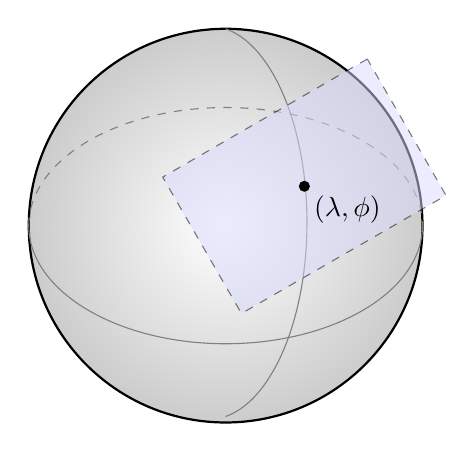
\begin{tikzpicture}[>=stealth]

    % 1. Define custom 3D projection vectors manually (Regular 2D coordinates)
    % This mimics a perspective view without the 3D library
    \coordinate (O) at (0,0);
    \def\R{2.5} % Radius of the sphere

    % 2. Draw the Sphere (Shading creates the 3D volume effect)
    \shade[inner color=white, outer color=gray!40] (O) circle (2.5);
    \draw[thick] (O) circle (\R);

    % 3. Draw Curvature Lines (Ellipses)
    % Equator-like curve
    \draw[gray, thin] (-\R,0) arc (180:360:{\R} and {0.6*\R});
    \draw[gray, dashed] (-\R,0) arc (180:0:{\R} and {0.6*\R});

    % Vertical curve (Longitude)
    \draw[gray, thin] (0,\R) arc (80:-80:{0.5*\R} and {\R});

    % 4. The Tangent Plane (A skewed quadrilateral)
    \coordinate (P) at (1, 0.5);
    \node [fill=blue!15, opacity=0.5, dashed, draw, shape=rectangle, minimum width=3cm, minimum height=2cm, anchor=center, rotate around={30:(P)}] at (P) {};

    % 5. Define the Target Point (P) on the surface
    \fill (P) circle (2pt) node[below right] {$(\lambda, \phi)$};

  \end{tikzpicture}

  \caption{Tangent space of $\S^2$}
  \label{fig:tangent_space_of_s2}
\end{figure}
